\chapter{Related Work}
\label{sec:related_work}

This chapter is based on a previous literature review and research proposal that have been prepared for this thesis. The literature review has been extended by recent publications and a clarification where this work contributes to the current state of the art.


\section{Sensor Modalities}

\subsection{2D Vision}
Early work in this area has been limited to single 2D perception capabilities. Thus, a common approach was to project known 3D objects into 2D and to compare these with perceived data from images. Chliveros et al. \cite{Chliveros2013}, Teuli\`ere et al. \cite{Teuliere2010}, Choi et al. \cite{Choi2012} and Azad et al. \cite{Azad2011} rely on an exact 3D model of an object for tracking and use a particle filter to maintain multiple hypotheses of the object's pose. These hypotheses are projected into a 2D plane (prediction step) and evaluated at the observation step. At this observation stage, the predicted edges of the 3D model in the 2D plane are compared with the linear edges and shapes extracted from the actual 2D sensor data. As a positive aspect, these approaches do not require range sensors but they do require detailed knowledge of the object's dimensions beforehand and do not exploit features from colour or texture, excluding Choi et al. which uses SIFT keypoints as initial pose estimation.

Recent template matching approaches explore special properties of boundary edges. Mu\~nos et al. \cite{Munoz2016} for example use HOG features (histograms of oriented gradients) to find corresponding edges between the template and the image. Cao et al. \cite{Cao2016} on the other side argue that HOG features lose pixel-level detail and instead use the cross-correlation between the Laplacian of Gaussian between templates and image patch. All template matching approaches have in common that they require a large database with templates of objects in all expected views.

\subsection{3D Vision}
\label{sec:3d_vision}

\paragraph{Single Articulated Objects}
With the advancement in range sensing and especially the availability of consumer depth sensors like the Kinect, similar approaches have been extended to 3D perception. Krull et al. \cite{Krull2015} apply a particle filter to estimate the object's pose in single images using RGB-D data by maintaining multiple hypotheses of the object pose. The observation distribution is generated from a discriminative learning method. Using example objects and an example background image, a random forest automatically learns useful features from the RGB-D data during a training phase. Once trained, the probability distribution of object class and coordinate location within the object is obtained for each new image.
%Their motion model assumes that an object continues its current motion and only changes by normally distributed translation and rotation.

The work of Shotton et al. \cite{Shotton2013} deals with complete body pose estimation and tracking of body parts. Instead of maintaining pose hypotheses of a single object, complete human skeleton hypotheses are evaluated. The observation distribution is generated by a discriminative classifier (random forest) using depth features for classifying 31 body parts. To achieve robustness and flexibility with their approach, a massive amount of training data is synthetically generated by rendering a body mesh at different sizes and with different joint configurations using motion capture.
The same combination of random forests and primitive depth features is applied by Widmaier et al. \cite{Widmaier2016} in a robotic manipulator context. However, they skip the intermediate task of classifying parts of the robot and instead predict its joint configuration directly.

A similar discriminative approach is used by Sharp et al. \cite{Sharp2015} to track articulated human hands.
For reinitialisation after tracking loss, the hierarchical distribution of hand poses is learned by a discriminative approach using synthetically generated training data.
Synthetic depth images are generated by sampling from a prior distribution of global hand translation and rotations, realistic wrist poses and six predefined finger and thumb states.
For finding the optimal hand configuration, they apply a mixture of particle swarm optimization (PSO) and genetic algorithms. In particle swarm optimization, particles represent solutions in the search space whose state is updated by the particle's own best known solution and by the swarm's global best known solution. PSO does not require the gradient of the optimized function.
Particles in PSO represent hypotheses as in particle filters, but their state is updated such that at least one particle's state is the global solution, whereas the current global solution of a particle filter is the expectation of the probability distribution formed by all particles (Monte Carlo expectation estimation).
At tracking loss, these hypotheses are reinitialized by the prediction of the discriminative method on the new depth input.
Each hypothesis of the particle swarm is evaluated by rendering its state and comparing it with the actual perceived sensor input.
To form the next generation of the particle swarm, particles with bad hypotheses are randomized and re-initialized.

\paragraph{Combined Object and Manipulator Tracking}
Pauwels et al. \cite{Pauwels2015} combined pose detection for reinitialization with pose tracking using dense motion and the information from depth data and colour. They rely on sparse SIFT keypoints sampled at equidistant viewpoints to obtain initial pose estimates and to reinitialize the tracker in case of tracking loss. The poses are continuously estimated using the shape and dense motion estimates of the object. This combination of both estimates enables them to cover difficult cases where the objected is blurred by motion or occluded (\cref{fig:simtrack_poses}).
The motion is represented as the optical flow on raw image data and on images which are augmented by objects rendered at their current estimated state.

\begin{figure}[h]
\centering
\subfloat[]{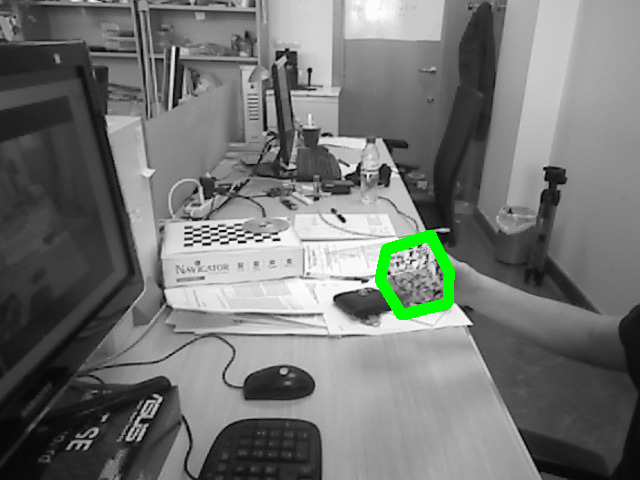
\includegraphics[width=0.33\textwidth]{images/related_work/dense_pose1.png} }
\subfloat[]{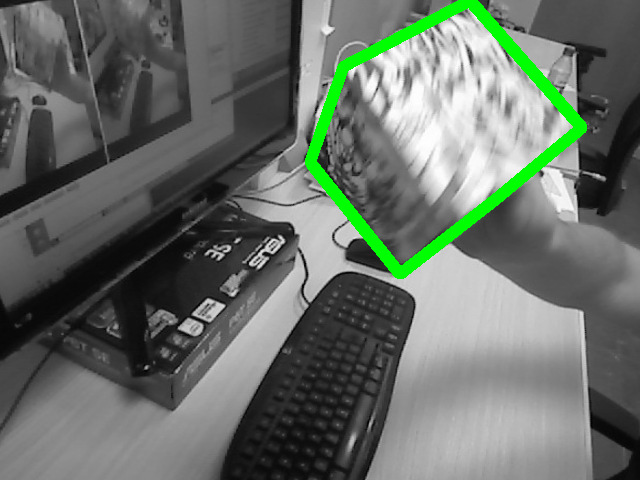
\includegraphics[width=0.33\textwidth]{images/related_work/dense_pose2.png} }
\subfloat[]{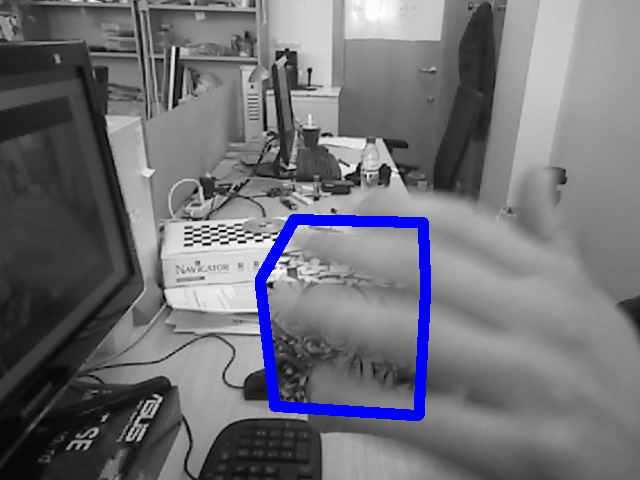
\includegraphics[width=0.33\textwidth]{images/related_work/sparse_pose1.png} }
\caption[SimTrack object tracking]{SimTrack: Examples of correct classified object poses. (a) and (b) using \textit{dense} estimation for small and blurry observations, (c) using \textit{sparse} keypoints for occluded observations. (Source: \cite{Pauwels2015}, figure 13)}
\label{fig:simtrack_poses}
\end{figure}

The multi-object tracking in SimTrack was extended for articulated objects \cite{Pauwels2014} by incorporating the pose updates into a kinematic chain with constraints. The pose of each rigid part is estimated independently from each other. The links between parts can be constrained to define free and static joints. The complete update of the kinematic chain takes into account the individual pose updates per part and the movement constraints of parts to each other.

SimTrack was further extended for joint object and manipulator tracking \cite{Pauwels2014b}, where the manipulator (arm and hand) is considered rigid after the joint values are used to articulate the model. As the approach relies on inaccurate joint encoder values, only the hand (which is assumed to be rigidly connected to the object) is tracked. Further, because the robot's surface is low textured, sparse features cannot be exploited.

The DART framework presented by Schmidt et al. \cite{Schmidt2015, Schmidt2015b} aims to provide a general framework for articulated tracking using depth sensors. DART assumes that the articulated model is given as a set of rigid objects with transformation from the kinematic chain and a local signed distance function that gives the distance of a point to the hull of the object (and is negative inside). The optimal joint configuration that minimizes the distance of the model to the observed point cloud is recovered by a gradient based optimization approach. \Cref{fig:dart_justin_est} shows this exemplary for hands and an object in a bimanual manipulation task.
Compared to particle filters, this does not maintain explicit hypotheses but optimizes on the distances.

\begin{figure}[h]
\centering
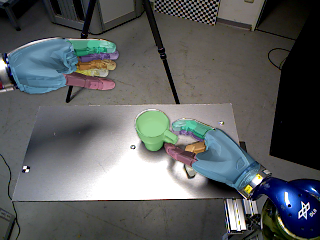
\includegraphics[width=0.5\textwidth]{images/related_work/dart_estim.png}
\caption[DART manipulator tracking]{DART: Depth based estimation of robot configuration projected on top of the perceived RGB image. (Source: \cite{Schmidt2015b}, figure 2)}
\label{fig:dart_justin_est}
\end{figure}

\subsection{Contact Sensors}

Schmidt et al. \cite{Schmidt2015b} and Koval et al. \cite{Koval2015} showed that contact sensing can be used to estimate the pose of an object or to reject visually proposed poses.
Koval et al. \cite{Koval2015} manipulated an object by pushing it over a planar surface and estimated its 2D position on the surface and orientation solely by contact sensors. They restrict their sensing to 9 strain gauges on the fingers and the palm of the hand, which only provides boolean information about contact (contact or no contact). By enhancing a particle filter to prevent particle starvation caused by the discrete states of the observation, they are able to estimate the position and orientation despite the low dimensionality of sensing.

As this approach does not scale from 3 DOF (2D position + 1D rotation) to 6DOF poses in 3D, contact sensing is best applied in conjunction with other sensing to eliminate unlikely hypotheses as in \cite{Schmidt2015b}.

\subsection{Kinematics and Constraints}

The work of Schmidt et al. in \cite{Schmidt2015} is extended in \cite{Schmidt2015b} to incorporate physical constraints, namely intersection of the manipulator with the object and contact with the object.
If the manipulated object is rigidly connected to a manipulator, the joint encoder values can be an important source to improve the object's pose estimate.

On the other hand, kinematic chains can be used to constrain estimated configurations to physically reasonable and likely values and eliminate unlikely hypotheses \cite{Shotton2013, Sharp2015}.
Whereas physical constraints are fixed, e.g. they always hold, kinematic constraints are soft, e.g. unlikely and unreasonable states might still occur.

\section{Real-Time Capabilities}

All of the particle filtering based approaches trade off the quality of the resulting pose estimation, as represented by the particles, with real-time constraints. An increasing number of particles cover a wider range of pose hypotheses but also increase the computation time.

Krull et al. \cite{Krull2015} however showed, that using a good proposal distribution can reduce the required amount of particles to achieve similar results compared to particle filters using generic distributions with many more particles.

A general and common solution to meet real-time constraints is the parallelisation of algorithms and offloading of computations to GPUs. Exemplary, the independent state updates for particles in a particle filter \cite{Choi2013} or the independent lookup of shortest distances of points to multiple models \cite{Schmidt2015} can easily be parallelized.


\section{Model-based and Model-free}

Tracking of rigid or articulated objects usually requires knowledge of the dimensions of the object or the manipulator beforehand. In contrast, there exist approaches that model manipulated objects and kinematic chains online during manipulation.

Krainin et al. \cite{Krainin2011} modelled objects online by tracking the manipulator and the object at the same time during a grasping task.
They address the issue of relying solely on either the object's appearance or the manipulator's joint values. Using only a single source of information can cause ambiguous and incorrect pose estimates for textureless and symmetric objects with lack of visual distinctive features.
By using multiple sources of information they are able to map highly symmetric 3D objects with lack of visual features and in presence of noisy joint values.

The issue of faulty or absent of joint encoder values is addressed by Sturm et al. \cite{Sturm2009}. In their work, the kinematic chain of an arm is learned from scratch and enables adaptation in cases of malfunction, e.g. if a joint is blocked or its strength decreases over time.
Si et al. \cite{Si2013} learn the variety of appearance of articulated objects as a hierarchical composition of parts as AND and OR nodes without providing labels. AND nodes define connection of parts, e.g. torso and limbs, and OR nodes represent different configurations of the same part. As a result, they can provide generic configurable templates for articulated objects.

The availability of accurate CAD models of robots and large online databases of 3D objects \cite{Firman2016, Singh2014} reduces the need to create models of common objects and enables the generation of huge synthetic training sets for discriminative approaches.

\section{Features}
Discriminative approaches, that learn the appearance of parts \cite{Shotton2013, Krull2015, Pauwels2015} or complete poses \cite{Sharp2015}, rely on manually designed features or keypoints like edges, SIFT \cite{Pauwels2015, Morwald2010} or depth features. In the RGB-D domain, where these features often neglect one of the channels, exploiting all the information is beneficial. Ren et al. \cite{Ren2012} applied kernel descriptor for RGB-D scene labelling and showed superior performance of RGB-D descriptors compared to RGB or depth only descriptors.

\paragraph{RGB-D Features and Descriptors}
Learned features not only provide a way to classify 3D objects by machine learning algorithms (e.g. SVM), but also provide interest points for pose estimation by homography.

Gupta et al. \cite{Gupta2014} combined feature learning on RGB-D data with pixel-wise classification for segmenting objects in depth data. Object region proposals from contours are classified by a linear SVM using RGB-D features learned by a Region-based Convolutional Neural Net (R-CNN). Classified regions are separated in foreground and background pixels using random forest and low-level features such as the pixel coordinate and depth, distance to ground plane and gravity vector. The foreground pixels are allocated to superpixel and classified into one of the many categories.

Blum et al. \cite{Blum2012} demonstrated an approach that learns RGB-D features in an unsupervised manner by convolutional k-means (CKM) around SURF interest points. Similar performance can be achieved by the hierarchical matching pursuit (HMP) approach \cite{Bo2013} in classification tasks. It was shown that HMP is applicable for pose estimation, achieving appropriable results for weak-symmetrical objects with unambiguous viewpoints.

\paragraph{Joint Detection}
In the work of Jain et al. \cite{Jain2015}, the location of joints in 2D image sequences are learned from labelled raw image data using a convolutional neural network (CNN) by only providing simple motion features. These positions can be used to infer a kinematic model of articulated objects.

Tompson et al. \cite{Tompson2014} applied a CNN to joint detection using depth data and are able to estimate the location of occluded parts without the need to provide joint connectivities from a kinematic model. They state that the inference of occluded parts is especially enabled by the hierarchical compound features learned in the CNN.

The spatial relation of compound parts is also exploited by Jiu et al. \cite{Jiu2014}. By learning a pixel-wise segmentation of human body parts incorporating spatial relation, the classification performance is increased with no additional computation costs during testing phase. As with most deep learning applications, they learn from raw depth data and do not require precomputed features.



\section{Conclusion from State-of-the-Art}
\label{sec:discussion}

The majority of the presented work in the field of articulated tracking applies a discriminative approach to depth sensor data. Because of the high variance in shape and viewpoint of the tracked objects, a very large amount of training data is required to learn a sufficient distribution of articulations. If the articulated objects are known beforehand and a large variety of sensor data is available or can be generated, this is a promising approach.

However, relying solely on either the learned representation of objects or the kinematics of the manipulator fails in cases of low structured objects (highly symmetric, lack of texture and visual features), non-reliable sensor data (occlusions, reflection of sunlight, shadows in depth data, non-IR-reflective surfaces) and noisy or improper calibrated joint encoders.

Tracking and pose estimation of multiple objects is only considered in a small fraction of the presented work. Most of the presented work focuses either on the tracking of rigid objects or the tracking of manipulators; or assumes no interaction of tracked objects.

This thesis contributes towards the optimal integration of prior information from joint position sensing in a setting where a robot is visually observing its own manipulator. We base our work on the optimization approach presented by Schmidt et al. \cite{Schmidt2015}, that in its original implementation uses solely depth observations to find an optimal robot configuration.
